\cotefile{156-4}
\scanpage{66}\mspage{65}
Ceci résulte du \deleted{\uline{C}4 et} cor. 1 et du

\uline{Lemme} Pour que $F$ soit de t. f.\inserted{(resp. fini)} il f et s que a) les $F_i$ le soient et b) Tous les $F_i$ sauf un nb fini sont $\varnothing$.

Notations $\pi_0(F)$ (NB Si $F\leq G$ on a $\pi_0(F)\longrightarrow\pi_0(G)$\deleted{\unsure{)}}, et transitivité) $\pi_0(M)$, $\pi_0^{\deleted{\unsure{\mathrm{cat}|\mathrm{act}}}!}(\unsure{.}\mathcal F)$. (\unsure{Attention}, le $\pi_0^{\unsure{\underset{\circ}{d}|!}}(\mathcal F)$ n'est pas le $\pi_0(F,\leq)$, mais le $\pi_0$ ``en tenant compte \unsure{du|des} Sup''. Si
% The following drawing preserves the two distinct pointers below the tuple.
% The two comparison forms occupy the same overwritten position in the manuscript.
\figure{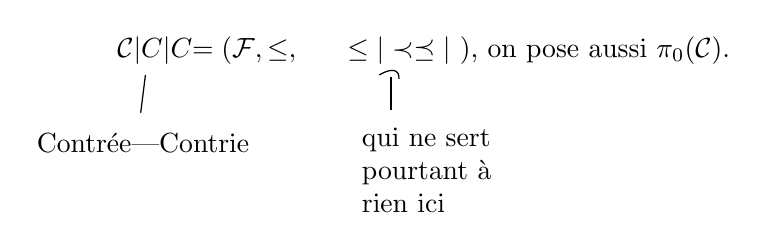
\begin{tikzpicture}[x=1cm,y=1cm]
\node[anchor=base] at (0,0) {$\unsure{\mathcal C|\mathscr C|C}$};
\node[anchor=base west] at (.35,0) {$=(\mathcal F,\leq,$};
\node[anchor=base] at (3.1,0) {$\deleted{\unsure{\leq|\prec}}\unsure{\preceq|\leqslant}$};
\node[anchor=base west] at (3.75,0) {$)$, on pose aussi $\pi_0(\mathcal C)$.};
\draw[line width=.45pt] (-.12,-.22)--(-.18,-.70);
\node[anchor=north] at (-.15,-.83) {\unsure{Contrée|Contrie}};
\draw[line width=.45pt] (3.0,-.67)--(3.0,-.24);
\draw[line width=.45pt] (2.85,-.22) .. controls (2.98,-.14) and (3.11,-.13) .. (3.10,-.27);
\node[anchor=north,align=left] at (3.45,-.77) {qui ne sert\\\deleted{\unsure{pourtant}} \unsure{à}\\rien ici};
\end{tikzpicture}}

Axiome renforcé

\uuline{C4 bis} Pour tout $(F_i)_i\in\prod\mathcal F_i$, $\deleted{\exists\unsure{\mathcal F|F}}$ $\exists F\in\mathcal F$ telle que $F\mid M_i=\deleted{\unsure{\mathcal F|F}}F_i$ pour $i\vdash I$.
% At the final F_i, the deleted form is overwritten by the live F, not a separate preceding group.

\uline{\unsure{Contrée|Contrie} résiduelle} \uline{Support} \uline{et} \uline{cosupport}

Soit $\deleted{\unsure{(F_i)\in\mathcal F|(H_i)\in\mathcal F}}$ $\Phi\subset\mathcal F$ un ens. de
% H_i is raised above the end of figures; the long slanted connector is distinct.
\figure{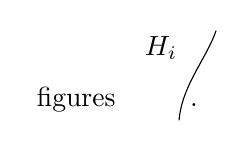
\begin{tikzpicture}[x=1cm,y=1cm]
\node[anchor=base west] at (0,0) {figures};
\node[anchor=base] at (1.70,.64) {\inserted{$H_i$}};
\draw[line width=.40pt] (1.93,-.18) .. controls (1.96,.25) and (2.28,.61) .. (2.40,.96);
\node[anchor=base] at (2.12,0) {.};
\end{tikzpicture}}
\deleted{On posera} Soit $F$ une figure. Pour \deleted{Cosupp. $\Phi$} que $F$ soit \unsure{disjointe|disjoint} de tous les $H_i$, il f et s. que ce soit le cas pour toutes les \unsure{strates} de $F$ (à cause de C3). \deleted{Posons} Posons
